\documentclass[a4paper,11pt,draft]{article}

\usepackage[finnish]{babel}
\usepackage[utf8]{inputenc}
\usepackage[margin=2cm]{geometry}
\usepackage{amsfonts,amsmath,amssymb,amsthm,enumitem}
\usepackage{pgf}
\usepackage{tikz}
\usetikzlibrary{arrows,automata}

\newtheorem*{claim}{Väite}
\newcommand{\set}[1]{{\left\{ #1 \right\}}}

\newenvironment{automata}[1][2.8]%
{\begin{tikzpicture}[->,>=stealth',shorten >=1pt,auto,node distance=#1cm,semithick]}%
{\end{tikzpicture}}

\begin{document}

\subsection*{582206 Laskennan mallit, syksy 2012\\
2. Harjoitusten malliratkaisut\\
{\rm
\begin{tabular}{ccc}
Jani Rahkola & ja & Juhana Laurinharju
\end{tabular}
}}

\begin{enumerate}
\item
  Olkoon kahden äärellisen automaatin $M_1$ ja $M_2$ tilat ja
  siirtymät seuraavat.
  
  \begin{enumerate}
  \item
    Mikä on kunkin automaatin aloitustila?
  \item
    Mitkä ovat hyväksyviä tiloja?
  \item
    Minkä tilajonon automaatit käyvät läpi syötteellä $aabb$?
  \item
    Hyväksyvätkö automaatit syötteen $aabb$?
  \item
    Hyväksyvätkö automaatit merkkijonon $\varepsilon$?
  \end{enumerate}

  \begin{tabular}{ccc}
  &
    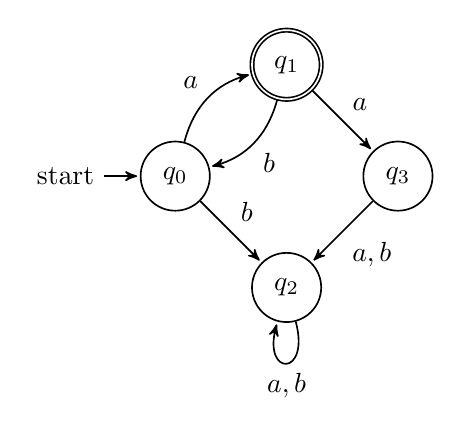
\begin{tikzpicture}[->,>=stealth',shorten >=1pt,auto,node distance=2.0cm,semithick]
      \node[initial,state]   (A)                    {$q_0$};
      \node[accepting,state] (B) [above right of=A] {$q_1$};
      \node[state]           (C) [below right of=A] {$q_2$};
      \node[state]           (D) [below right of=B] {$q_3$};

      \path (A) edge [bend left]  node {$a$} (B)
                edge              node {$b$} (C)
            (B) edge              node {$a$} (D)
                edge [bend left]  node {$b$} (A)
            (C) edge [loop below] node {$a,b$} (C)
            (D) edge              node {$a,b$} (C);
    \end{tikzpicture}
    &
    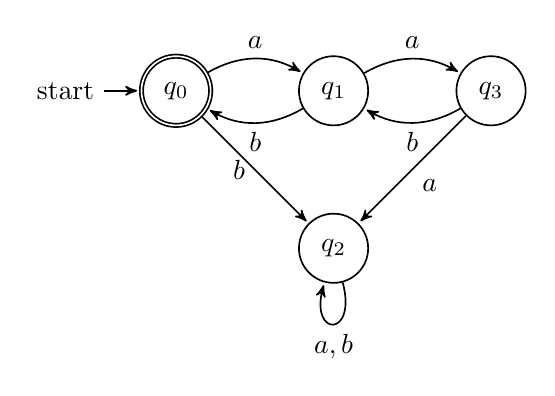
\begin{tikzpicture}[->,>=stealth',shorten >=1pt,auto,node distance=2.0cm,semithick]
      \node[initial,accepting,state]   (A)              {$q_0$};
      \node[state]                     (B) [right of=A] {$q_1$};
      \node[state]                     (C) [below of=B] {$q_2$};
      \node[state]                     (D) [right of=B] {$q_3$};

      \path (A) edge [bend left]   node {$a$}        (B)
                edge               node [left] {$b$} (C)
            (B) edge [bend left]   node {$a$}        (D)
                edge [bend left]   node {$b$}        (A)
            (C) edge [loop below]  node {$a,b$}      (C)
            (D) edge               node {$a$}        (C)
                edge [bend left]   node {$b$}        (B);
    \end{tikzpicture}
    \\
        & $M_1$             & $M_2$ \\
    (a) & $q_0$             & $q_0$ \\
    (b) & $\set{q_1}$       & $\set{q_0}$ \\
    (c) & $q_0q_1q_3q_2q_2$ & $q_0q_1q_3q_1q_0$ \\
    (d) & ei                & kyllä \\
    (e) & ei                & kyllä


\end{tabular}
\item Olkoon äärellisen automaatin $M$ formaali kuvaus
  $(\set{q_1,q_2,q_3,q_4,q_5}, \set{u,d}, \delta, q_3, \set{q_3})$ missä
  siirtymäfunktion määrittelee taulukko:
\[
\begin{array}{c|cc}
    & u   & d   \\ \hline
q_1 & q_1 & q_2 \\
q_2 & q_1 & q_3 \\
q_3 & q_2 & q_4 \\
q_4 & q_3 & q_5 \\
q_5 & q_4 & q_5
 \end{array} 
\]
Piirrä automaatti $M$ (tilat ja siirtymät).

\begin{automata}
  \node[state]                   (q1)               {$q_1$};
  \node[state]                   (q2)  [left of=q1] {$q_2$};
  \node[state,initial above,accepting] (q3)  [left of=q2] {$q_3$};
  \node[state]                   (q4)  [left of=q3] {$q_4$};
  \node[state]                   (q5)  [left of=q4] {$q_5$};


  \path (q1) edge [loop right] node {$u$} (q1)
             edge [bend right] node {$d$} (q2)
        (q2) edge [bend right] node {$u$} (q1)
             edge [bend right] node {$d$} (q3)
        (q3) edge [bend right] node {$u$} (q2)
             edge [bend right] node {$d$} (q4)
        (q4) edge [bend right] node {$u$} (q3)
             edge [bend right] node {$d$} (q5)
        (q5) edge [bend right] node {$u$} (q4)
             edge [loop left]  node {$d$} (q5);

\end{automata}

\item Minkälaisia merkkijonoja eli sanoja seuraavat äärelliset automaatit hyväksyvät?

\begin{tabular}{cccc}
(a) & 
\begin{tabular}{c}
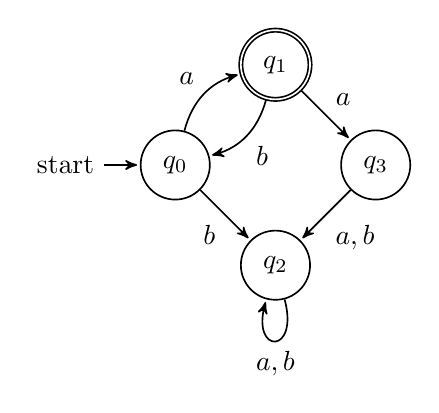
\begin{tikzpicture}[->,>=stealth',shorten >=1pt,auto,node distance=1.8cm,semithick]
 %\tikzstyle{every state}=[fill=red,draw=none,text=white]

 \node[initial,state]  (q0)                     {$q_0$};
 \node[state,accepting](q1) [above right of=q0] {$q_1$};
 \node[state]          (q2) [below right of=q0] {$q_2$};
 \node[state]          (q3) [above right of=q2] {$q_3$};

 \path (q0) edge [bend left]  node       {$a$} (q1)
            edge              node [swap]{$b$} (q2)
       (q1) edge              node       {$a$} (q3)
            edge [bend left] node        {$b$} (q0)
       (q2) edge [loop below] node {$a,b$} ()
       (q3) edge             node {$a,b$} (q2);
\end{tikzpicture} 
\end{tabular}
& (b) &
\begin{tabular}{c}
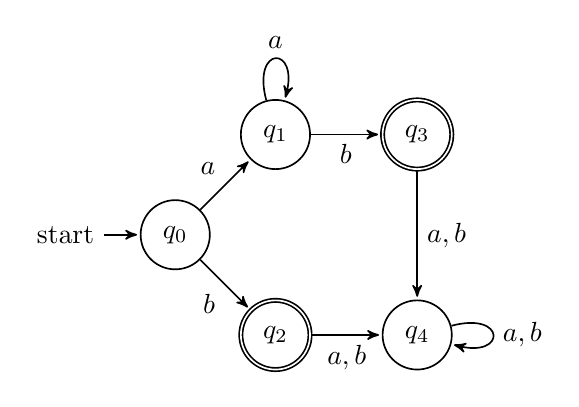
\begin{tikzpicture}[->,>=stealth',shorten >=1pt,auto,node distance=1.8cm,semithick]
 %\tikzstyle{every state}=[fill=red,draw=none,text=white]

 \node[initial,state]   (q0)                     {$q_0$};
 \node[state]           (q1) [above right of=q0] {$q_1$};
 \node[state,accepting] (q2) [below right of=q0] {$q_2$};
 \node[state,accepting] (q3) [right of=q1]       {$q_3$};
 \node[state]           (q4) [right of=q2]       {$q_4$};

 \path (q0) edge              node       {$a$}   (q1)
            edge              node [swap]{$b$}   (q2)
       (q1) edge [loop above] node       {$a$}   ()
            edge              node [swap]{$b$}   (q3)
       (q2) edge              node [swap]{$a,b$} (q4)
       (q3) edge              node       {$a,b$} (q4)
       (q4) edge [loop right] node       {$a,b$} ();    
\end{tikzpicture}
\end{tabular}
\end{tabular}

\begin{tabular}{cccc}
(c) &
\begin{tabular}{c}
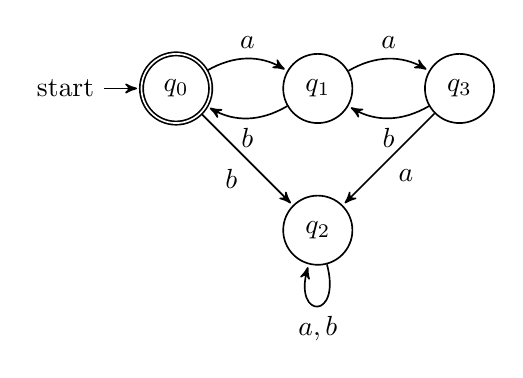
\begin{tikzpicture}[->,>=stealth',shorten >=1pt,auto,node distance=1.8cm,semithick]
 %\tikzstyle{every state}=[fill=red,draw=none,text=white]

 \node[initial,state,accepting]
              (q0)               {$q_0$};
 \node[state]           (q1) [right of=q0] {$q_1$};
 \node[state] (q2) [below of=q1] {$q_2$};
 \node[state] (q3) [right of=q1] {$q_3$};

 \path (q0) edge [bend left]  node       {$a$}   (q1)
            edge              node [swap]{$b$}   (q2)
       (q1) edge [bend left]  node       {$a$}  (q3)
            edge [bend left]  node       {$b$}   (q0)
       (q2) edge [loop below] node       {$a,b$} ()
       (q3) edge              node       {$a$}   (q2)
       (q3) edge [bend left]  node       {$b$} (q1);
\end{tikzpicture}
\end{tabular}
& (d) &
\begin{tabular}{c}
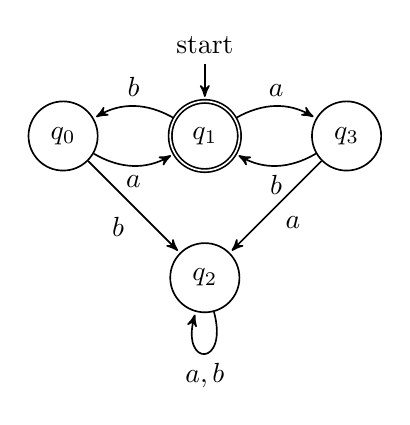
\begin{tikzpicture}[->,>=stealth',shorten >=1pt,auto,node distance=1.8cm,semithick]
 %\tikzstyle{every state}=[fill=red,draw=none,text=white]

 \node[state] (q0)               {$q_0$};
 \node[state,initial above,accepting]
              (q1) [right of=q0] {$q_1$};
 \node[state] (q2) [below of=q1] {$q_2$};
 \node[state] (q3) [right of=q1] {$q_3$};

 \path (q0) edge [bend right]  node [swap]{$a$}   (q1)
            edge              node [swap]{$b$}   (q2)
       (q1) edge [bend left]  node       {$a$}  (q3)
            edge [bend right]  node [swap]{$b$}   (q0)
       (q2) edge [loop below] node       {$a,b$} ()
       (q3) edge              node       {$a$}   (q2)
       (q3) edge [bend left]  node       {$b$} (q1);
\end{tikzpicture}
\end{tabular}
\end{tabular}

\begin{tabular}{cccc}
(e) &
\begin{tabular}{c}
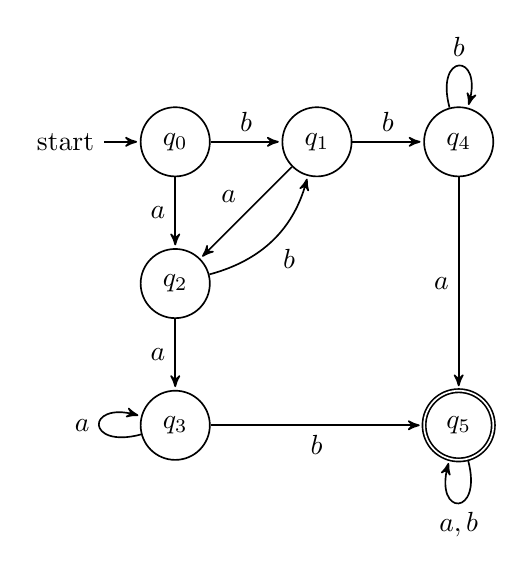
\begin{tikzpicture}[->,>=stealth',shorten >=1pt,auto,node distance=1.8cm,semithick]
 %\tikzstyle{every state}=[fill=red,draw=none,text=white]

 \node[state,initial] (q0)               {$q_0$};
 \node[state]       (q1) [right of=q0] {$q_1$};
 \node[state]       (q2) [below of=q0] {$q_2$};
 \node[state]       (q3) [below of=q2] {$q_3$};
 \node[state]       (q4) [right of=q1]  {$q_4$};
 \node              (qx)[below of=q4] {};
 \node[state,accepting](q5)[below of=qx] {$q_5$};
 
 \path (q0) edge              node [swap] {$a$}   (q2)
            edge              node        {$b$}   (q1)
       (q1) edge              node [swap] {$a$}   (q2)
            edge              node        {$b$}   (q4)
       (q2) edge              node [swap] {$a$}   (q3)
            edge [bend right] node [swap] {$b$}   (q1)
       (q3) edge [loop left]  node        {$a$}   (  )
       (q3) edge              node [swap] {$b$}   (q5)
       (q4) edge              node [swap] {$a$}   (q5)
       (q4) edge [loop above] node        {$b$}   (  )
       (q5) edge [loop below] node        {$a,b$} (  );
\end{tikzpicture}
\end{tabular}
\end{tabular}

\begin{tabular}{cl}
  (a) & $\set{a} \circ \set{ba}^* = a(ba)^*$ \\
  (b) & $\set{a}^* \circ \set{b} = a^*b$ \\
  (c) & $(\set{a} \circ \set{ab}^* \circ \set{b})^* = (a(ab)^*b)^*$ \\
  (d) & $\set{ab}^* \cup \set{ba}^* = (ab)^* | (ba)^*$ \\
  (e) & $\set{a,b}^* \circ \set{aab,bba} \circ \set{a,b}^* = (a|b)^*(aab|bba)(a|b)^*$
\end{tabular}

\item Piirrä äärelliset automaatit tiloineen ja siirtymänuolineen seuraaville kielille.
\begin{enumerate}
\item $L = \set{w \in \set{a, b}^* \mid \mbox{$w$ sisältää ainakin yhden $a$:n}}$

    \begin{automata}
        \node[initial,state]   (q1)               {$q_1$};
        \node[accepting,state] (q2) [right of=q1] {$q_2$};

        \path (q1) edge [loop above] node {$b$}   (  )
                   edge              node {$a$}   (q2)
              (q2) edge [loop above] node {$a,b$} (  );
    \end{automata}

\item $L = \set{w \in \set{a, b}^* \mid \mbox{$w$ alkaa $b$ tai $ab$:llä}}$

    \begin{automata}[2]
        \node[initial,state]   (q1)                     {$q_1$};
        \node[state]           (q2) [above right of=q1] {$q_2$};
        \node[accepting,state] (q3) [below right of=q2] {$q_3$};
        \node[state]           (q4) [above of=q2]       {$q_4$};
        
        \path (q1) edge              node {$a$} (q2)
                   edge              node {$b$} (q3)
              (q2) edge              node {$b$} (q3)
                   edge              node {$a$} (q4)
              (q3) edge [loop right] node {$a,b$} ()
              (q4) edge [loop above] node {$a,b$} ();
    \end{automata}

\item $L = \set{w \in \set{a,b}^*  \mid \mbox{$w$ loppuu $aa$:han}}$

    Suunnitellun automaatin olisi tarkoitus "muistaa", ollaanko nähty nolla,
    yksi vai ainakin kaksi $a$-merkkiä. Luodaan siis automaatille tilat
    jokaista kolmea vaihtoehtoa varten. Alkutilassa ei olla vielä nähty yhtään
    $a$:ta. Tilassa $q_a$ ollaan nähty yksi $a$ ja tilassa $q_{aa}$ ollaan
    nähty ainakin kaksi $a$:ta.

    \begin{automata}
        \node[initial,state]   (qe)                {$q_\varepsilon$};
        \node[state]           (qa)  [below of=qe] {$q_a$};
        \node[accepting,state] (qaa) [right of=qa] {$q_{aa}$};

        \path (qe)  edge [loop above] node        {$b$} (  )
                    edge [bend left]  node        {$a$} (qa)
              (qa)  edge [bend left]  node        {$b$} (qe)
                    edge              node        {$a$} (qaa)
              (qaa) edge [loop right] node        {$a$} (  )
                    edge              node [swap] {$b$} (qe);
    \end{automata}

\item
  $L = \set{w \in \set{a,b}^* \mid \mbox{$w$ sisältää merkkijonon
    $abab$ }}$

  \begin{automata}
    \node[initial,state]   (qe)                    {$q_\varepsilon$};
    \node[state]           (qa)    [right of=qe]   {$q_a$};
    \node[state]           (qab)   [right of=qa]   {$q_{ab}$};
    \node[state]           (qaba)  [right of=qab]  {$q_{aba}$};
    \node[accepting,state] (qabab) [right of=qaba] {$q_{abab}$};

    \path (qe)    edge [loop above] node        {$b$}   ()   
                  edge              node        {$a$}   (qa)   
          (qa)    edge [loop below] node        {$a$}   ()     
                  edge              node        {$b$}   (qab)  
          (qab)   edge [bend right] node [swap] {$b$}   (qe)   
                  edge              node        {$a$}   (qaba) 
          (qaba)  edge [bend left]  node        {$a$}   (qa)       
                  edge              node        {$b$}   (qabab)
          (qabab) edge [loop above] node        {$a,b$} ();
  \end{automata}

\item
  $L = \set{w \in \set{a,b}^* \mid \mbox{jokaisen $w$:ssä olevan $a$:n
    edessa on $b$}}$
  
  \begin{automata}
    \node[initial,accepting,state] (q1)                     {$q_1$};
    \node[accepting,state]         (q2) [above right of=q1] {$q_2$};
    \node[state]                   (q3) [below right of=q1] {$q_3$};

    \path (q1) edge              node        {$a$}   (q3)
               edge [bend right] node [swap] {$b$}   (q2)
          (q2) edge [bend right] node [swap] {$a$}   (q1)
               edge [loop right] node        {$b$}   ()
          (q3) edge [loop right] node        {$a,b$} ();
  \end{automata}

\end{enumerate}

\item
  Olkoon kielet $A$ ja $B$ säännöllisiä. Todista että joukkoerotus $A
  - B$ tuottaa säännöllisen kielen luentokalvojen yhdisteen esimerkin
  mukaisesti. Piirrä myös pieni esimerkki automaateista $L(M_1)=A$,
  $L(M_2)= B$ ja $L(M_{A-b})=A-B$.

  Koska $A$ ja $B$ ovat säännöllisiä, on olemassa äärelliset
  automaatit $M_A = (Q_A, \Sigma, \delta_A, s_A, F_A)$ ja $M_B = (Q_B,
  \Sigma, \delta_B, s_B, F_B)$ jotka tunnistavat kielet $A$ ja $B$.
  Siis $L(M_A) = A$ ja $L(M_B) = B$.

  Määritellään automaatti $M_{A-B} = (Q_{A-B}, \Sigma, \delta_{A-B},
  s_{A-B}, F_{A-B})$ missä
%
  \begin{align*}
    Q_{A-B} &= Q_A \times Q_B \\
    \delta_{A-B}((q_A, q_B), a) &= (\delta_A(q_A,a), \delta_B(q_B,a)) \\
    s_{A-B} &= (s_A, s_B) \\
    F_{A-B} &= \set{(q_A, q_B) \in Q_{A-B} \mid q_A \in F_A \text{ ja
      } q_B \notin F_B} = F_A \times (Q_B - F_B)
  \end{align*}
%
  FIXME: Motivaatio
%
  \begin{claim}
    Yllä määritelty automaatti $M_{A-B}$ tunnistaa kielen $A - B$.
    Siten kieli $A - B$\\ on säännöllinen.
  \end{claim}
%
  \begin{proof}
    Olkoon $w \in \Sigma^*$. Nyt
%
    \begin{equation*}
      w = w_1 \ldots w_n.
    \end{equation*}
%
    Määritellään tilajonot
%
    \begin{align*}
      r &= r_1 \ldots r_{n+1} \text{ ja } \\
      p &= p_1 \ldots p_{n+1}
    \end{align*}
%
    joiden läpi automaatit $M_A$ ja $M_B$ kulkevat merkkijonon $w$
    aikana siten, että
%
    \begin{align*}
      r_1     &= s_A              & p_1    &= s_B \\
      r_{i+1} &= \delta_A(r_i,w_i) & p_{i+1} &= \delta_B(p_i, w_i).
    \end{align*}
%
    \begin{center}
    \begin{automata}[1.3]
      \tikzstyle{every state}=[fill=none,draw=none,text=black,minimum
        size=0.8cm,inner sep=0cm]
      \node[state]                     (r1)                   {$r_1$};
      \node[state,node distance=1.7cm] (r2)   [right of=r1]   {$r_2$};
      \node[state]                     (dots) [right of=r2]   {$\ldots$};
      \node[state]                     (rn)   [right of=dots] {$r_{n+1}$};
      \node[state,node distance=0.5cm] (sa)   [below of=r1]   {$s_A$};
      \node[state,node distance=0.5cm] (dsa)[below of=r2] {$\delta_A(s_A, w_1)$};

        \path (r1)   edge [bend left] node {$w_1$} (r2)
              (r2)   edge [bend left] node {$w_2$} (dots)
              (dots) edge [bend left] node {$w_n$} (rn);
    \end{automata}
    \end{center}
    FIXME: tee tästä makro niin voi piirtää vastaavan kuvan myös kahelle
    muulle jonolle

%
    Automaatti $M_A$ kulkee syötteellä $w$ tilajonon $r$ ja automaatti
    $M_B$ tilajonon $p$ läpi. Siis esimerkiksi automaatti $M_A$
    siirtyy merkillä $w_i$ tilasta $r_i$ tilaan $r_{i+1}$.

    Määritellään myös vastaavasti jono
% 
   \begin{equation*}
      q = q_{1} \ldots q_{n+1}
    \end{equation*}
% 
   jonka läpi automaatti $M_{A-B}$ kulkee syötteellä $w$. Nyt siis
%
    \begin{align*}
      q_1 &= s_{A-B} = (s_A, s_B) = (r_1,p_1) \\
      q_{i+1} &= \delta_{A-B}(q_i, w_i).
    \end{align*}
%
    Intuitiivisesti näyttäisi siltä, että $q_i = (r_i,p_i)$, sillä
%
    \begin{align*}
      q_1 &= (r_1, p_1) \\
      q_2 &= \delta_{A-B}(q_1, w_1) \\
          &= (\delta_A(r_1, w_1), \delta_B(p_1, w_1) \\
          &= (r_2, p_2) \\
      \ldots &
    \end{align*}
%
    Näytetään tämä todeksi induktiolla.
%
    \begin{claim}
      $q_i = (r_i,p_i)$ tai $n+1 < i$
    \end{claim}
%
    \begin{proof}
      \begin{description} \item[]
        \item[Alkuaskel] määritelmän nojalla $q_1 = (r_1,p_1)$.
        \item[Induktioaskel]
          \begin{description}\item[]
            \item[Induktio-oletus] $i > n+1$ tai $q_i = (r_1,p_i)$
            \item[Induktioaskeleen väite] $i+1 > n+1$ tai $q_{i+1} =
            (r_{i+1}, p_{i+1})$

            \item[Induktioaskeleen todistus] \mbox{} %tyhjä kappale

            Jos $i \ge n+1$, niin $i+1 > n+1$. Tarkastellaan siis tapausta
            $i < n+1$. Nyt
%
            \begin{align*}
              q_{i+1} &= \delta_{A-B}(q_i, w_i)
                         &\text{$q_{i+1}$:n määritelmä}\\
                      &= \delta_{A-B}((r_i, p_i), w_i)
                         &\text{induktio-oletus} \\
                      &= (\delta_A(r_i, w_i), \delta_B(p_i, w_i))
                         &\text{$\delta_{A-B}$:n määritelmä}\\
                      &= (r_{i+1}, p_{i+1})
                         &\text{$r_{i+1}$:n ja $p_{i+1}$:n määritelmät.}
            \end{align*}
          \end{description}
      \end{description}
    \end{proof}
%

    Automaatti $M_{A-B}$ hyväksyy merkkijonon $w$ jos ja vain jos
    $q_{n+1} \in F_{A-B}$. Näytetään nyt, että $M_{A-B}$ hyväksyy merkkijonon
    $w$ täsmälleen silloin kun $w$ kuuluu kieleen $A -B$.
%
    \begin{align*}
      q_{n+1} \in F_{A-B}
      &\Leftrightarrow (r_{n+1}, p_{n+1}) \in F_{A-B} \\
      &\Leftrightarrow r_{n+1} \in F_A \text{ ja } p_{n+1} \notin F_B \\
      &\Leftrightarrow w \in A \text{ ja } w \notin B \\
      &\Leftrightarrow w \in A - B.
    \end{align*}
%
    Siis kieli $A - B$ on säännöllinen.
  \end{proof}

\end{enumerate}
\end{document}
